\chapter{Аналитический раздел}

В аналитическом разделе выполнено изучение предметной области, представлено формальное описание данных, выполнен анализ существующих моделей и методов организации хранения данных в базе знаний.

\section{Постановка задачи}

Необходимо спроектировать и реализовать базу данных, содержащую информацию о киберспортивных матчах и командах в дисциплине Dota 2. Следует разработать интерфейс, который позволит работать с этой базой данных: добавлять, удалять и редактировать информацию, составлять отчеты по периодам, задаваемым пользователем, с их графическим представлением. Требуется предусмотреть наличие ролей модератора и администратора, осуществляющих контроль за добавлением новых турниров, регистрацией новых команд и обновлением текущих составов.

\section{Актуальность проекта}

С каждым годом призовые фонды турниров становятся все больше. Более того, киберспортивные первенства проходят даже в пределах конкретных организаций, школ, колледжей, университетов и других объединений, которые в свою очередь нельзя подробно изучить в одном месте.

Российская команда Team Spirit стала победителем The International 10, что существенным образом сказалось на популярности и интересе к киберспортивной составляющей Dota 2 \cite{teamspirit}.

Таким образом, разрабатываемое приложение предложит удобный инструмент для просмотра статистики по киберспортивным турнирам, с возможностями добавления своих и составления отчетов за выбранный период.

\section{Предметная область}

\subsection{Краткое описание игрового процесса}

Dota 2 представляет собой соревновательную командную игру с RPG (англ. Role-Playing Game --- ролевая игра) элементами типа MOBA (<<многопользовательская онлайновая боевая арена>>). Две соревнующиеся команды Света (англ. The Radiant) и Тьмы (англ. The Dire) состоят из пяти игроков каждая. Главной целью игры в Dota 2 является уничтожение вражеской крепости (англ. Ancient). Каждая из крепостей защищается несколькими башнями, расположенными вдоль трех линий обороны. Вместо построения собственной армии как в классических RTS играх (англ. Real Time Strategy --- Стратегии реального времени), каждый игрок управляет одним уникальным героем с отличительными умениями, узнаваемой внешностью, силами, слабостями и уникальным стилем игры \cite{dota2}.


Каждый из игроков выполняет определенную роль на протяжении матча,  как например <<керри>> (англ. Carry) или <<саппорт>> (англ. Support), и герои могут по своим характеристикам лучше подходить для той или иной роли. Во время игры герой имеет возможность зарабатывать опыт и золото, которое можно тратить на покупку предметов, которые позволяют усилить одну или несколько характеристик персонажа: урон по другим героям, восстановление здоровья или потенциал уничтожения вражеских строений. 

Если очки здоровья героя снижаются до нуля — например, его одолевает в бою вражеский герой --- герой в течение некоторого короткого времени считается <<погибшим>>; по окончании этого времени герой вновь появляется рядом с крепостью, и управляющий им игрок может возобновить игру. Убийство врага позволяет получить большое количество дополнительного золота и опыта.

\subsection{Dota Pro Circuit}

Dota Pro Circuit --- профессиональные турниры организуются компанией Valve и её партнёрами, для определения команд, которые получат прямые приглашения на The International (главный турнир года).

Заработанные за сезон баллы будут определять статус команды перед The International и её шансы на получение прямого приглашения \cite{dpc}.

\section{Обзор существующих сервисов}

Следует отметить, что существуют сервисы, которые агрегируют, систематизируют и визуализируют информацию о киберспортивных турнирах.

DOTABUFF является крупнейшим сервисом для сбора и анализа матчевой статистики, в том числе о профессиональных матчах. Однако, данный сервис доступен только на английском языке и помимо киберспортивной информации имеет множество дополнительной, которая несколько осложняет взаимодействие (см. рисунок \ref{fig:dotabuff}).

\begin{figure}[h!btp]
	\centering
	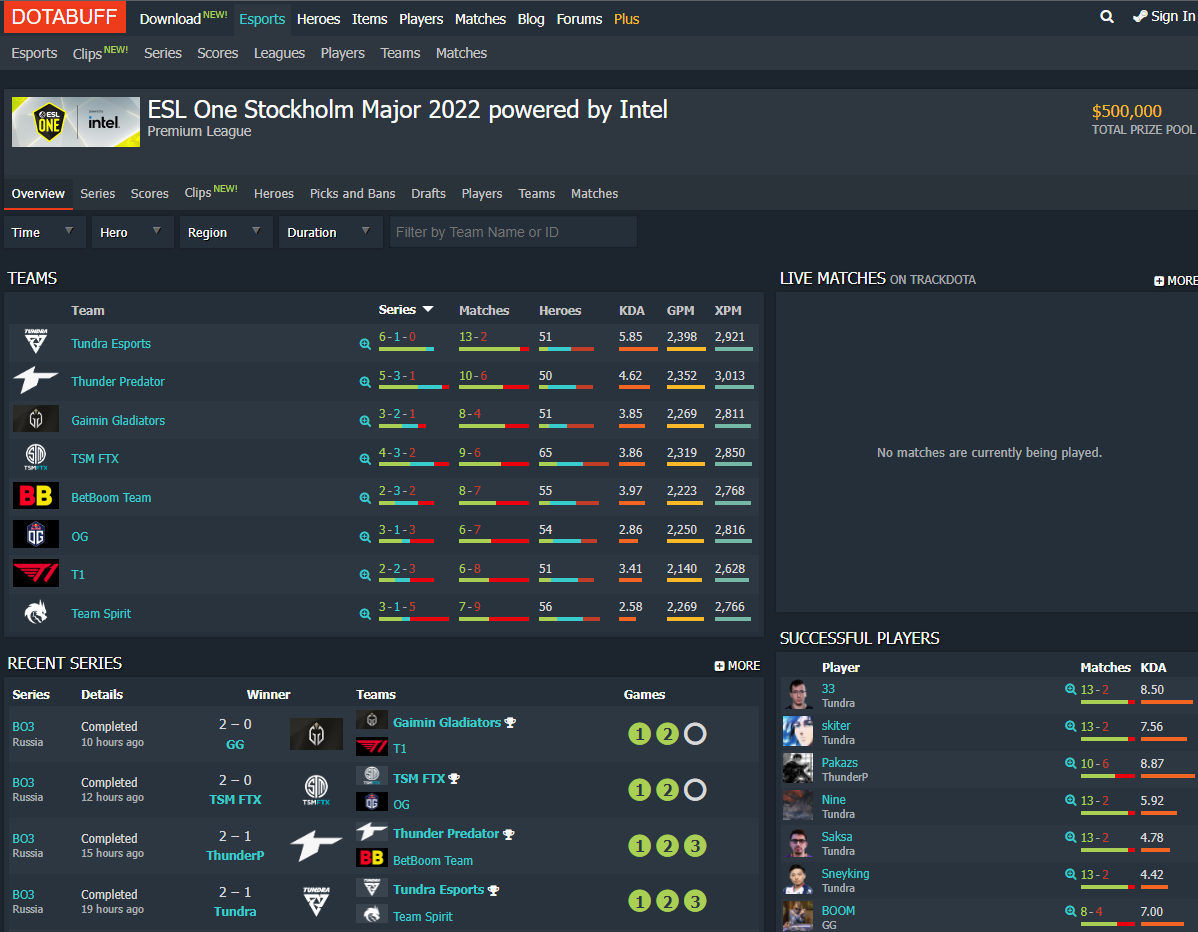
\includegraphics[width=450pt]{inc/img/dotabuff.png}
	\caption{Портал dotabuff.com}
	\label{fig:dotabuff}	
\end{figure}

OpenDota --- это проект энтузиастов с открытым исходным кодом, собирающий данные Dota 2. Сервис предоставляет веб-интерфейс для обычных пользователей, так же как API для разработчиков с возможностью интеграции в сторонние приложения. Большим плюсом является возможность детального изучения матча с автоматизированной аналитикой и советами  (см. рисунок \ref{fig:opendota}) \cite{opendota}.

\begin{figure}[h!btp]
	\centering
	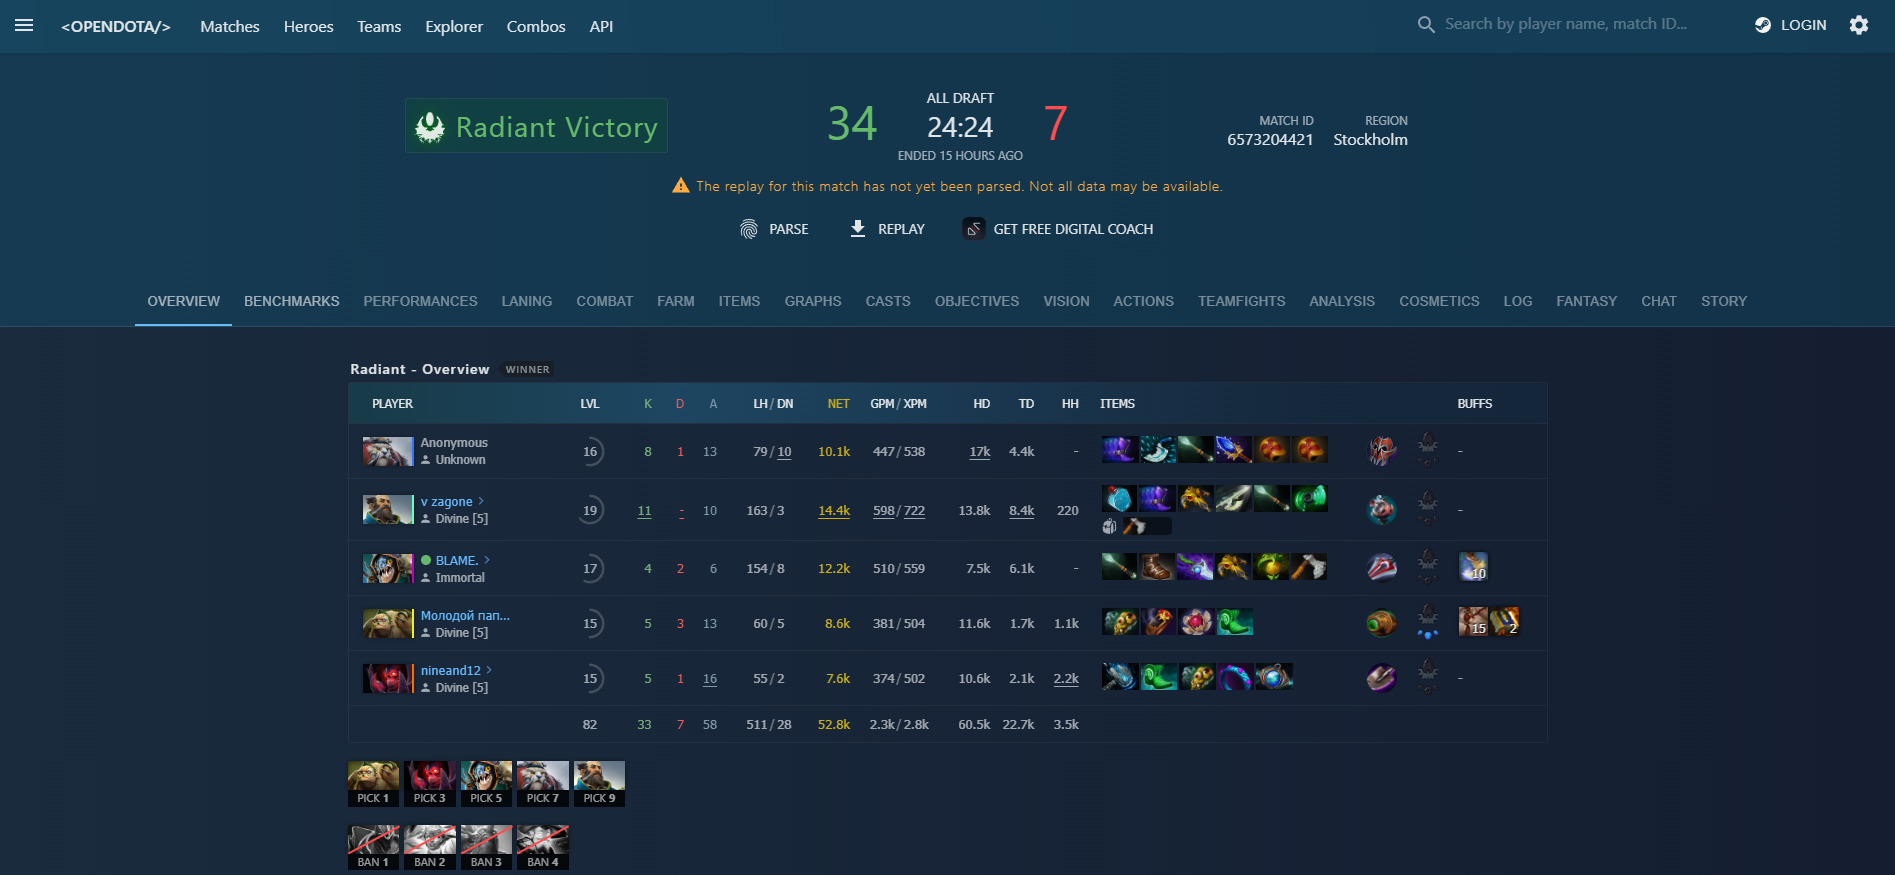
\includegraphics[width=450pt]{inc/img/opendota.png}
	\caption{Портал opendota.com}
	\label{fig:opendota}	
\end{figure}

\newpage

На рисунке \ref{fig:cybersport} представлен портал cybersport.ru. Данный сервис специализируется на широком круге киберспортивных дисциплин. Портал позволяет смотреть матчи в прямом эфире, следить за турнирной сеткой, читать новости о профессиональных игроках и командах, но не дает пользователю подробной статистики и послематчевой аналитики. Доступность на русском языке выгодно выделяет сервис на фоне конкурентов.

\begin{figure}[h!btp]
	\centering
	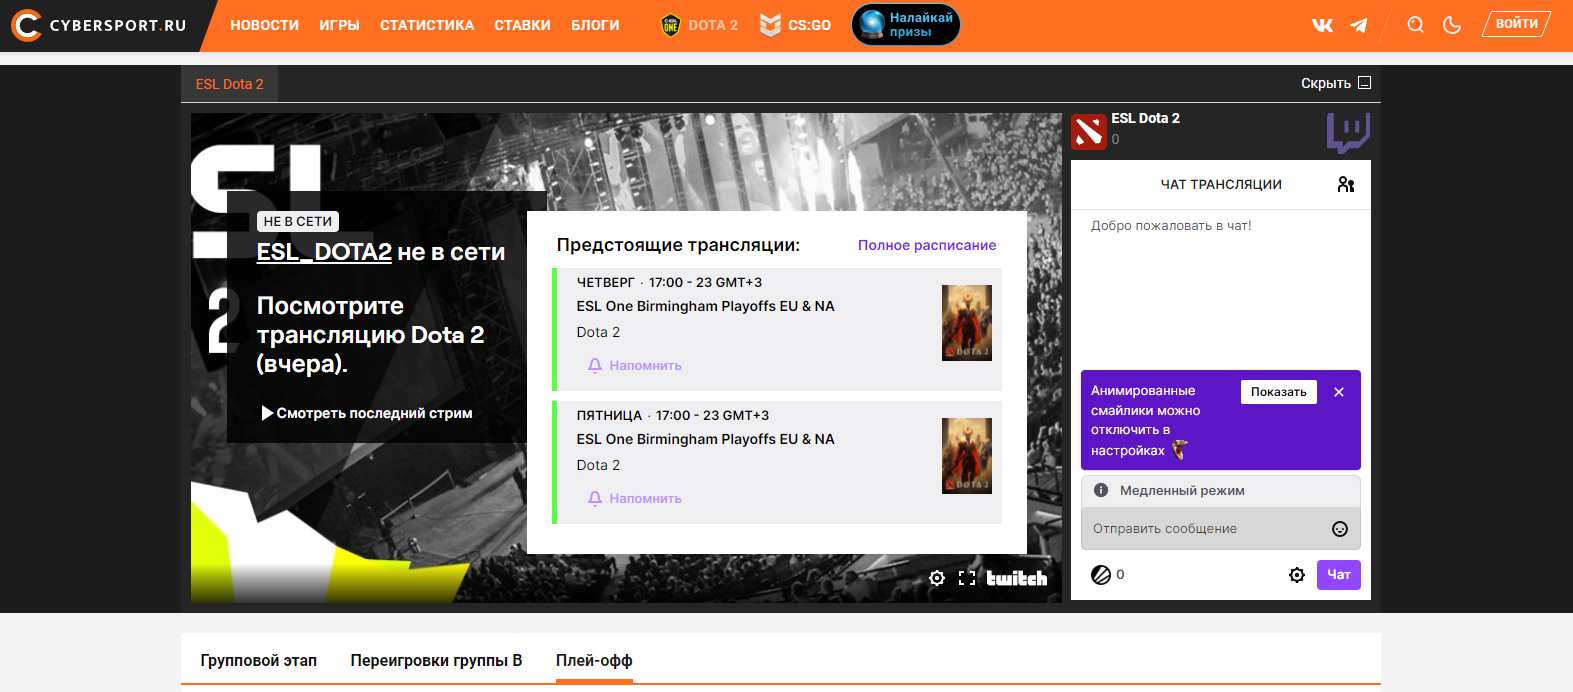
\includegraphics[width=450pt]{inc/img/cybersport.png}
	\caption{Портал cybersport.ru}
	\label{fig:cybersport}	
\end{figure}

Таким образом, на основе рассмотренных сервисов можно составить сравнительную таблицу \ref{tabular:services}.

\begin{table}[h!]
	\centering
	\caption{\label{tabular:services}Сравнительная таблица сервисов}
	\begin{tabular}{|p {5 cm}|p {3cm}|p {3cm}|p {3.5 cm}|}
		\hline
		\textbf{} & \textbf{DOTABUFF} & \textbf{OpenDota} & \textbf{cybersport.ru} \\ \hline
		\textbf{Открытый исходный код} & - & + & - \\ \hline
		\textbf{Доступность} & По подписке & Бесплатно & С рекламой \\ \hline
		\textbf{Послематчевая статистика} & + & + & - \\ \hline
		\textbf{Турниры} & - & - & + \\ \hline
		\textbf{Язык} & Английский & Английский & Русский \\ \hline
		\textbf{Наличие desktop-приложения} & + & - & - \\ \hline
	\end{tabular}
	
\end{table}

Ни один из представленных сервисов не обладает desktop-приложением, возможностью просмотра турниров и доступностью на русском языке. Разрабатываемое ПО должно соответствовать этим требованиям.

\newpage

\section{Типы пользователей}

Разрабатываемая система ориентирована на многопользовательское использование, следовательно, важным является разделение пользователей по ролям и соответствующему им функционалу (таблица \ref{tabular:users_info}).

\begin{table}[h!]
	\centering
	\caption{\label{tabular:users_info}Типы пользователей и доступный им функционал}
	\begin{tabular}{|p{5 cm}|p{10 cm}|}
		\cline{1-2}
		\textbf{Тип пользователя}  & \textbf{Доступный функционал}                                                                           \\ \cline{1-2}
		Неавторизованный & Регистрация, авторизация \\ \cline{1-2}
		Клиент & Просмотр информации о киберспортивных матчах, прошедших турнирах, составах команд, сведений о игроках и сводной статистики за заданный период\\ \cline{1-2}
		Модератор & Просмотр информации о киберспортивных матчах, прошедших турнирах, составах команд, сведений о игроках и сводной статистики за заданный период
		\newline
		Операции доступа, изменения и удаления информации в базе знаний \\ \cline{1-2}
		Администратор & Просмотр информации о киберспортивных матчах, прошедших турнирах, составах команд, сведений о игроках и сводной статистики за заданный период
		\newline
		Операции доступа, изменения и удаления информации в базе знаний
		\newline 
		Добавление и удаление пользователей, изменение типа существующего пользователя \\ \cline{1-2}
	\end{tabular}%
\end{table}

Возможные варианты взаимодействия с системой описаны при помощи UseCase--диаграммы, которая приведена на рисунке \ref{fig:use_case}.

\begin{figure}[h!btp]
	\centering	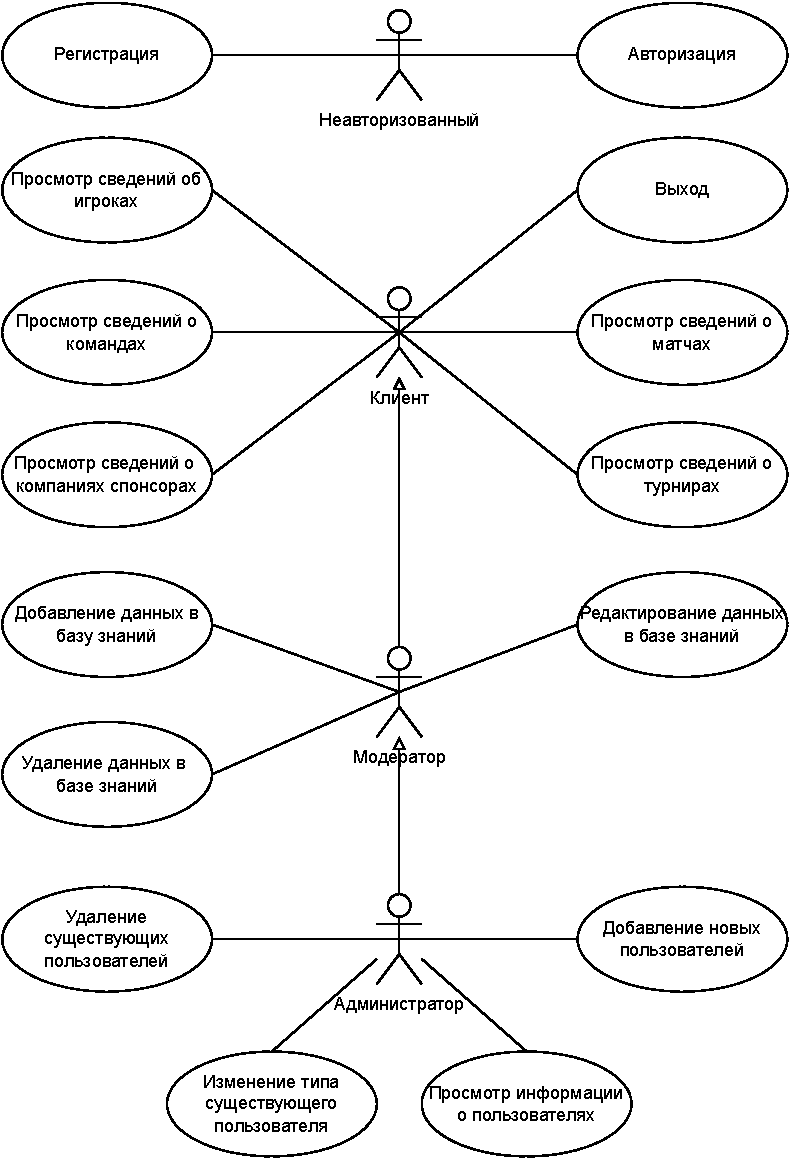
\includegraphics[width=450pt]{inc/diag/use_case.pdf}
	\caption{UseCase-диаграмма}
	\label{fig:use_case}	
\end{figure}

\newpage

\section{Формализация данных}

База данных должна хранить информацию о: 
\begin{itemize}
	\item турнирах;
	\item компаниях-спонсорах;
	\item командах;
	\item игроках;
	\item матчах;
	\item пользователях.
\end{itemize}

В таблице \ref{tabular:data_info} описано формальное представление данных и сведения, которые они содержат.

\begin{table}[h!]
	\centering
	\caption{\label{tabular:data_info}Данные и сведения о них}
	\begin{tabular}{|p{3 cm}|p{12 cm}|}
		\cline{1-2}
		\textbf{Данные}  & \textbf{Сведения}                                                                           \\ \cline{1-2}
		Турнир           & Название, уровень, призовой фонд, дата, время и место проведения, количество DPC очков   \\ \cline{1-2}
		Компания-спонсор & Название, страна, вебсайт, ежегодная выручка, область деятельности                \\ \cline{1-2}
		Команда          & Название, дата создания, контактный e-mail, общий заработок, регион, уровень             \\ \cline{1-2}
		Игрок            & Псевдоним, имя, дата рождения, страна, личный рейтинг, игровая позиция, сигнатурный герой   \\ \cline{1-2}
		Матч             & Продолжительность, победитель, герои, соотношение убийств, смертей и помощи, общая ценность, опыт и золото в минуту, урон\\ \cline{1-2}
		Пользователь     & Логин, пароль, права доступа, e-mail, имя                                                 \\ \cline{1-2}
	\end{tabular}%
\end{table}

На основе выделенных данных и сведений, которые они содержат, следует составить диаграмму в нотации Чена, описывающую сущности исследуемой системы, а также их взаимодействие (рисунок \ref{fig:chen}).

\newpage

\begin{figure}[h!btp]
	\centering
	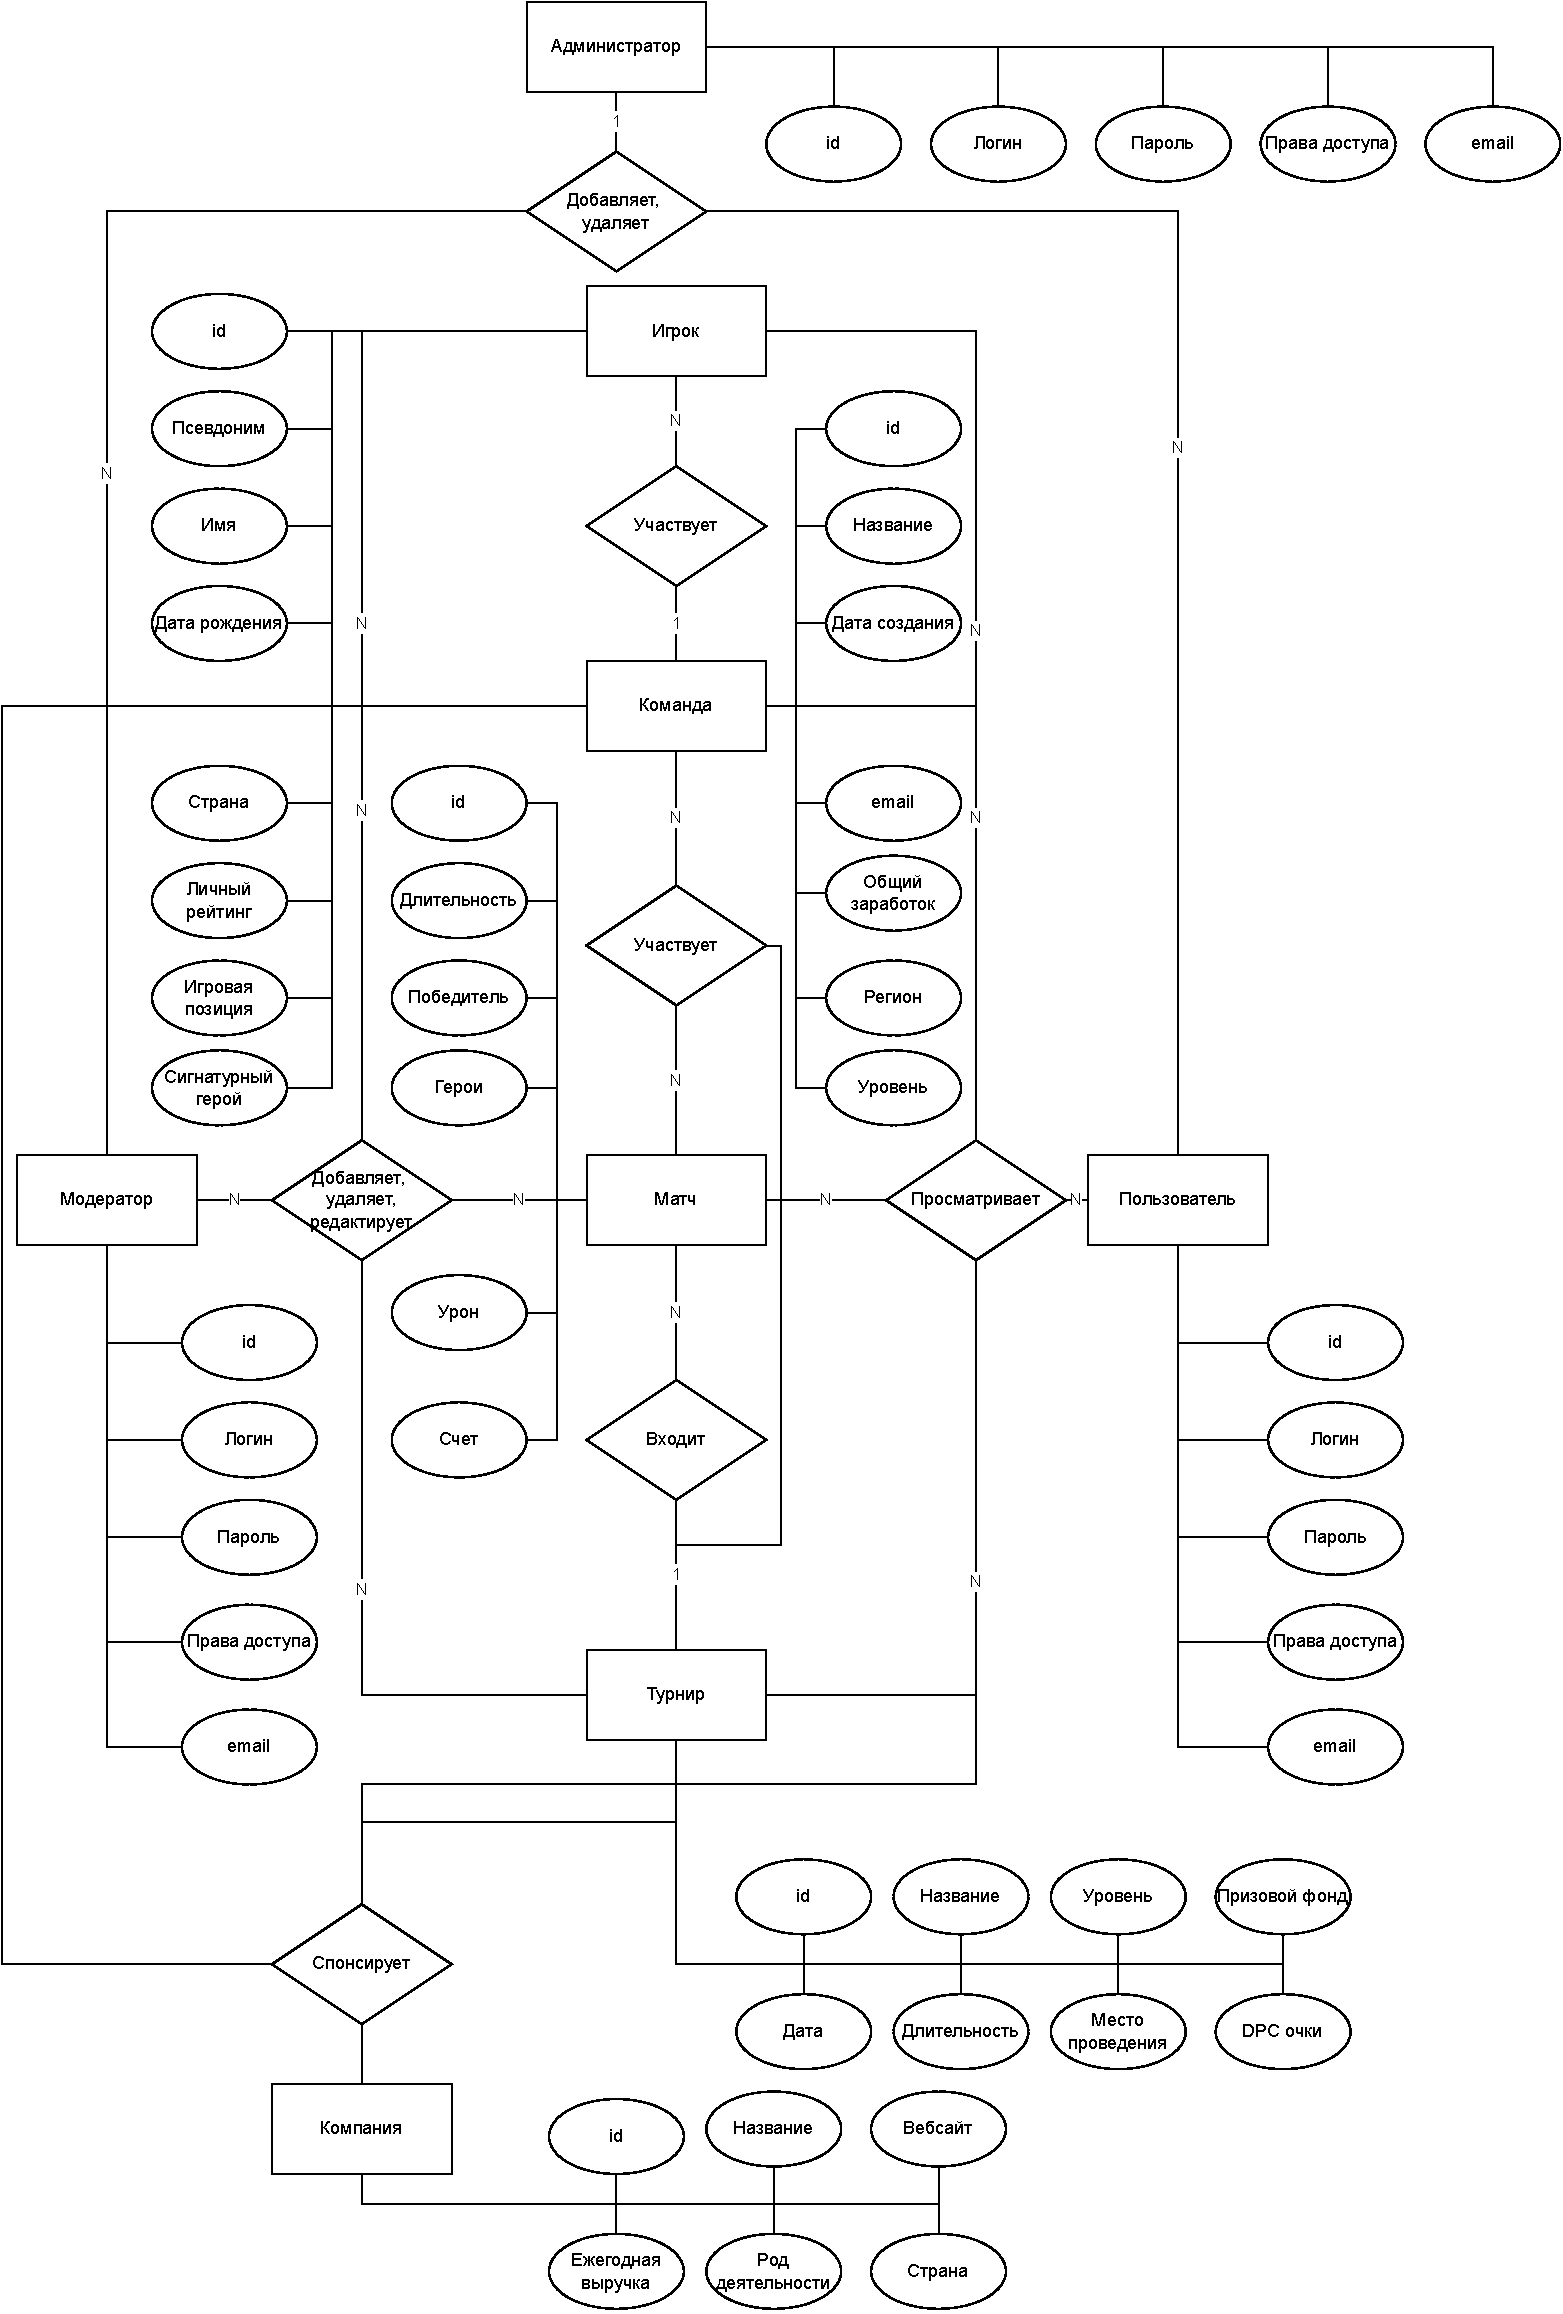
\includegraphics[width=450pt]{inc/diag/chen.pdf}
	\caption{Диаграмма сущность--связь}
	\label{fig:chen}	
\end{figure}

\newpage


\section{Выводы}

В данном разделе было выполнено изучение предметной области, представлено формальное описание данных, возможные варианты взаимодействия с системой описаны при помощи UseCase--диаграммы, а также составлена диаграмма сущность--связь предметной области. 


